% !TeX program = lualatex
% !BIB program = biber
% Lualatex is important to render TTF fonts; with pdflatex it's just the regular one
% ratio 16:9 -- https://tex.stackexchange.com/questions/14336/

% compile two versions, inspired by https://tex.stackexchange.com/a/1501
% use the script "compile-pdf.sh"
\newif\ifhandout
% if flags.tex does not exist, create an empty file to be able to compile in TeXstudio
\input{flags}

\ifhandout
\documentclass[12pt,aspectratio=169,handout]{beamer}
\else
\documentclass[12pt,aspectratio=169]{beamer}
\fi



% TODO change "leftfootertext" to your liking
\newcommand{\leftfootertext}{\insertsubtitle}  % just the \title{} text by default
%\newcommand{\leftfootertext}{AI is all you need | Dr.\ Maria Mustermann}  % Your name, for instance


% ------- RUB specifics ----------
% adjust for 16:9
% https://tex.stackexchange.com/questions/354022/modifying-the-margins-of-all-slides-in-beamer
\setbeamersize{text margin left=0.3cm,text margin right=4.5cm} 


% use Metropolis as the basis theme
\usetheme[subsectionpage=progressbar]{metropolis}
% blocks with background globally
\metroset{block=fill}


\usepackage{fontspec}
% RUB fonts need to be installed
% 'UprightFont = * Light' makes sure that the base font is RubFlama Light, which looks
% lighter than RubFlama Regular (would be too thick for slides)
\setsansfont[Scale=MatchLowercase, UprightFont = * Light, BoldFont = * Bold]{RubFlama}
%\setsansfont{Arial} % Open source alternative if you don't have RubFlama

% RUB color scheme
% Dark blue: 0; 53; 96; #003560
\definecolor{RUBDarkBlue}{RGB}{0, 53, 96}

% Light yellow (table fill, etc.); 238; 250; 196; #EEFAC4
\definecolor{RUBLightYellow}{RGB}{238, 250, 196}

%Light green: 141; 174; 16
\definecolor{RUBLightGreen}{RGB}{141, 174, 16}


\setbeamercolor{titlelike}{fg=RUBDarkBlue}
\setbeamercolor{subtitle}{fg=RUBLightGreen}
\setbeamercolor{separation line}{fg=RUBLightGreen}
\setbeamercolor{frametitle}{bg=white, fg=RUBDarkBlue}

% horizontal line on title page and sections
\setbeamercolor{alerted text}{fg=RUBLightGreen}


% Adjust footer bottom (too large by default)
\setbeamertemplate{footline}{%
  \begin{beamercolorbox}[wd=\textwidth, sep=2ex]{footline}%
    \usebeamerfont{page number in head/foot}%
    \usebeamertemplate*{frame footer}
    \hfill%
    \usebeamertemplate*{frame numbering}
  \end{beamercolorbox}%
}


% Lab name, numbering, etc. in footer
\setbeamertemplate{frame numbering}{TrustHLT --- Prof.\ Dr.\ Ivan Habernal \hspace*{1ex} \includegraphics[width=7em]{img/rub-logo.pdf}\hspace*{1ex}}

\setbeamertemplate{frame footer}{\hspace*{1ex}\insertframenumber \hspace*{2ex} \leftfootertext}

% adjust the background to be completely white
\setbeamercolor{background canvas}{bg=white}

% logos on the title page
\titlegraphic{%
	\begin{picture}(0,0)
		\put(435,0){\makebox(0,0)[rt]{\includegraphics[width=7em]{img/rub-logo.pdf}}}
		\put(435,-170){\makebox(0,0)[rt]{\includegraphics[width=4em]{img/logo-trusthlt.pdf}}}
		\put(435,-196){\makebox(0,0)[rt]{\includegraphics[width=9em]{img/logo-rctrust.pdf}}}
	\end{picture}%
}


% show TOC at every section start
\AtBeginSection{
	\frame{
		\vspace{2em}
		\sectionpage
		\hspace*{2.2em}\begin{minipage}{10cm}
			\tableofcontents[currentsection]
		\end{minipage}
	}
}

% TOC without subsection
\setcounter{tocdepth}{1} % only-- part,chapters,sections 

% bullet points: rectangles
\useinnertheme{rectangles}
\setbeamercolor{itemize item}{fg=RUBLightGreen}
\setbeamercolor{itemize subitem}{fg=RUBLightGreen}
% enumerate: blue background for better readability
\setbeamercolor{item projected}{bg=RUBDarkBlue}

% make boxes (example, block, etc.) background lighter for readability
\setbeamercolor{block title}{%
	use=normal text,
	fg=normal text.fg,
	bg=normal text.bg!90!fg % lighter background in block title
}
\setbeamercolor{block body}{
	use={block title, normal text},
	bg=block title.bg!30!normal text.bg % lighter background in block body
}


% RUB colors in blocks
\setbeamercolor{block title alerted}{%
	use={block title, alerted text},
	bg=RUBDarkBlue,
	%fg=RUBLightYellow % looks bad
	fg=white % better contrast
}

\setbeamercolor{block title example}{%
	use={block title, example text},
	fg=RUBLightGreen
}


% ------- end of RUB specifics ----------

% all itemize with pause by default
%\beamerdefaultoverlayspecification{<+->}


% typeset mathematics on serif
\usefonttheme[onlymath]{serif}

% better bibliography using biber as backend
\usepackage[natbib=true,backend=biber,style=authoryear-icomp,maxbibnames=30,maxcitenames=9,uniquelist=false,giveninits=true,doi=false,url=false,dashed=false,isbn=false]{biblatex}
% shared bibliography
\addbibresource{../../nlpwdl-bibliography.bib}
% disable "ibid" for repeated citations
\boolfalse{citetracker}



\usepackage{xspace}


% for derivatives, https://tex.stackexchange.com/a/412442
\usepackage{physics}

\usepackage{tikz}
\usetikzlibrary{matrix, positioning}
\usetikzlibrary{angles,quotes} % for angles
\usetikzlibrary{backgrounds} % background
\usetikzlibrary{decorations.pathreplacing} % curly braces
\usetikzlibrary{calligraphy}
\usetikzlibrary{calc} % for neural nets

% for plotting functions
\usepackage{pgfplots}
\usepgfplotslibrary{dateplot}

% sub-figures
\usepackage{caption}
\usepackage{subcaption}

% book tabs
\usepackage{booktabs}


% argmin, argmax
\usepackage{amsmath}
\DeclareMathOperator*{\argmax}{arg\!\max}
\DeclareMathOperator*{\argmin}{arg\!\min}
% softmax
\DeclareMathOperator*{\softmax}{soft\!\max}
% Mask
\DeclareMathOperator*{\mask}{mask}

% bold math
\usepackage{bm}

% for \mathclap
\usepackage{mathtools}

% algorithms
\usepackage[noend]{algpseudocode}


% for neurons and layers in tikz
\tikzset{
	neuron/.style={draw, rectangle, inner sep=2pt, minimum width=0.75cm, fill=blue!20},
	param/.style={draw, rectangle, inner sep=2pt, minimum width=0.75cm, fill=green!20},
	constant/.style={draw, rectangle, inner sep=2pt, minimum width=0.75cm, fill=black!15},
	% for citation nodes right top
	ref/.style={anchor = north east, text width=7.8cm, yshift=-1.3cm, xshift=-0.2cm, scale=0.5},
	state/.style={rectangle, inner sep=2pt, minimum width=0.75cm, fill=black!5},
}

% added in lecture 10
\tikzset{
	mtx/.style={
		matrix of math nodes,
		left delimiter={[}, right delimiter={]}
	},
	hlt/.style={opacity=0.1, line width=4 mm, line cap=round},
	hltr/.style={opacity=0.5, rounded corners=2pt, inner sep=-1pt}
}

% for strike-through text (added in Lecture 06)
\usepackage[normalem]{ulem}

% added in Lecture 7
% RNN
\DeclareMathOperator*{\rnn}{RNN}
% RNN star
\DeclareMathOperator*{\rnnstar}{RNN^{*}}
% bi-RNN
\DeclareMathOperator*{\birnn}{biRNN}


% added in Lecture 9
\usetikzlibrary{fit} % for hightligting by calling "fit"

% algorithms
\usepackage[noend]{algpseudocode}



\title{Natural Language Processing with Deep Learning}
\subtitle{Lecture 4 --- Text classification with log-linear models}
\date{November 14, 2024}
\author{Prof.\ Dr.\ Ivan Habernal}
\institute{
\texttt{www.trusthlt.org} \\
Trustworthy Human Language Technologies Group (TrustHLT) \\
Ruhr University Bochum \& Research Center Trustworthy Data Science and Security}


\begin{document}

\maketitle

\section{Backpropagation}

\subsection{Efficient computation of gradient}

\begin{frame}{Working example}
	
	$$
	e = (a + b)(b + 1)
	$$
	
	Compute gradient wrt.\ $a$ and $b$
	
	\bigskip
	
	\pause
	
	\begin{block}{This one is easy by hand, but that's not the point}
		$$
		e = (a + b)(b + 1) = ab + a + b^2 + b
		$$
		$$
		\pdv{e}{a} = b + 1 \qquad \pdv{e}{b} = a + 2b + 1
		$$
	\end{block}
	
\end{frame}



\begin{frame}{Add some intermediate variables and function names}
	\includegraphics[width=1.1\linewidth]{img/backprop01.pdf}
\end{frame}

\begin{frame}{Build computational graph and evaluate (forward step)}
	\includegraphics[width=1.1\linewidth]{img/backprop02.pdf}
	
	
	\begin{tikzpicture}[overlay, remember picture] 
		\node at (current page.north east)[anchor = north east, text width=4cm, yshift=-1.3cm] {\scriptsize \textbf{Important:} $a, b$ will be some concrete real numbers, therefore $r, s, e$ will be concrete real numbers too! \par};
	\end{tikzpicture}	
	
\end{frame}


\begin{frame}{Computational graph}
	\begin{itemize}
		\item DAG --- directed acyclic graph (not necessarily a tree!)
		\item Each node --- a differentiable function with arguments
		\item Leaves --- variables (e.g., $a, b$) or constants
		\item Arrows --- Function composition
	\end{itemize}
	
	\begin{figure}
		\includegraphics[width=0.75\linewidth]{img/parent-child.pdf}
		\caption{$r, s$ are parents of $b$; $a, b$ are children (arguments) of $r$}
	\end{figure}
	
	
	
\end{frame}

\begin{frame}{Goal: $\pdv{e}{a}$ and $\pdv{e}{b}$ (gradient), but let's do $\pdv{e}{\star}$ for every node}
	\includegraphics[width=1.1\linewidth]{img/backprop03.pdf}
\end{frame}

\begin{frame}{Since $e = r \cdot s$, partial derivatives are easy: $\pdv{e}{r} = s$ and $\pdv{e}{s} = r$}
	\includegraphics[width=1.1\linewidth]{img/backprop04.pdf}
	
	\begin{tikzpicture}[overlay, remember picture] 
		\node at (current page.north east)[anchor = north east, text width=4cm, yshift=-1.7cm] {\scriptsize \textbf{Sanity check:} $r, s$ are some concrete real numbers, therefore $\pdv{e}{r}$ and $\pdv{e}{s}$ will be concrete real numbers too! \par};
	\end{tikzpicture}
\end{frame}

\begin{frame}{Proceed to next child $r$ and compute $\pdv{e}{r}$ -- use chain rule!}
	\includegraphics[width=1.1\linewidth]{img/backprop05.pdf}
	
	
\end{frame}

\begin{frame}{Proceed to next child $s$ and compute $\pdv{e}{s}$ -- use chain rule!}
	\includegraphics[width=1.1\linewidth]{img/backprop06.pdf}
\end{frame}

\begin{frame}{Since $r = a + b$, partial derivatives are easy: $\pdv{r}{a} = 1$ and $\pdv{r}{b} = 1$}
	\includegraphics[width=1.1\linewidth]{img/backprop07.pdf}
\end{frame}

\begin{frame}{Proceed to next child $a$ and compute $\pdv{e}{a}$ -- use chain rule!}
	\includegraphics[width=1.1\linewidth]{img/backprop08.pdf}
\end{frame}

\begin{frame}{Since $s = b + 1$, partial derivatives are easy: $\pdv{s}{b} = 1$}
	\includegraphics[width=1.1\linewidth]{img/backprop09.pdf}
\end{frame}

\begin{frame}{Proceed to $b$ and compute $\pdv{e}{b}$ -- use multivariate chain rule!}
	\includegraphics[width=1.1\linewidth]{img/backprop10.pdf}
\end{frame}


\begin{frame}{Goal: $\nabla e = \left( \pdv{e}{a}; \pdv{e}{b} \right)$ --- we computed it for concrete $a$ and $b$!}
	\includegraphics[width=1.1\linewidth]{img/backprop10.pdf}
\end{frame}


\begin{frame}{Generic node in a computational graph}
	
	
	
	
	
	
	\begin{figure}
		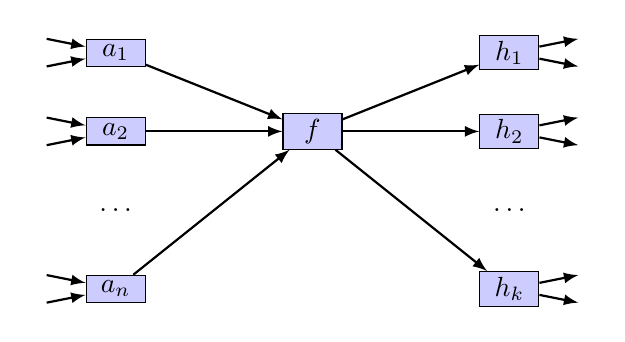
\begin{tikzpicture}	
			%\node (a1) [draw, circle, inner sep=0pt, minimum width=0.75cm, fill=green!20] {$a_1$};
			\node (a1) [neuron] {$a_1$};
			\node (a2) [neuron, below of=a1] {$a_2$};
			\node (dots1) [below of=a2] {$\ldots$};
			\node (an) [neuron, below of=dots1] {$a_n$};
			
			\node (f) [neuron, right of=a2, xshift=1.5cm] {$f$};
			
			\node (h2) [neuron, right of=f, xshift=1.5cm] {$h_2$};
			\node (h1) [neuron, above of=h2] {$h_1$};
			\node (dots2) [below of=h2] {$\ldots$};
			\node (hk) [neuron, below of=dots2] {$h_k$};
			
			% inputs
			\node (a1in1) [left of=a1, yshift=0.2cm] {};
			\node (a1in2) [left of=a1, yshift=-0.2cm] {};
			
			\node (a2in1) [left of=a2, yshift=0.2cm] {};
			\node (a2in2) [left of=a2, yshift=-0.2cm] {};
			
			\node (anin1) [left of=an, yshift=0.2cm] {};
			\node (anin2) [left of=an, yshift=-0.2cm] {};
			
			% outputs
			\node (h1o1) [right of=h1, yshift=0.2cm] {};
			\node (h1o2) [right of=h1, yshift=-0.2cm] {};
			
			\node (h2o1) [right of=h2, yshift=0.2cm] {};
			\node (h2o2) [right of=h2, yshift=-0.2cm] {};
			
			\node (hko1) [right of=hk, yshift=0.2cm] {};
			\node (hko2) [right of=hk, yshift=-0.2cm] {};
			
			
			\begin{scope}[thick, black, ->, >=latex]
				\draw (a1) -- (f);
				\draw (a2) -- (f);
				\draw (an) -- (f);
				\draw (f) -- (h1);
				\draw (f) -- (h2);
				\draw (f) -- (hk);
				
				\draw (a1in1) -- (a1);
				\draw (a1in2) -- (a1);
				\draw (a2in1) -- (a2);
				\draw (a2in2) -- (a2);
				\draw (anin1) -- (an);
				\draw (anin2) -- (an);
				
				\draw (h1) -- (h1o1);
				\draw (h1) -- (h1o2);
				\draw (h2) -- (h2o1);
				\draw (h2) -- (h2o2);
				\draw (hk) -- (hko1);
				\draw (hk) -- (hko2);
			\end{scope}	
		\end{tikzpicture}
		
		
		\caption{A generic node of a computation graph. Node $f$ has many inputs, its output
			feeds into many nodes, and each of its inputs and outputs may also have many inputs
			and outputs.}
	\end{figure}
	

	\begin{tikzpicture}[overlay, remember picture] 
		\node at (current page.north east)[ref] {Adapted from \fullcite[p.~265]{Kun.2020} \par};
	\end{tikzpicture}
	
\end{frame}


\begin{frame}{Generic node in a computational graph $f(a_1, \ldots, a_n)$}
	
	\begin{figure}
		\scalebox{0.6}{%
			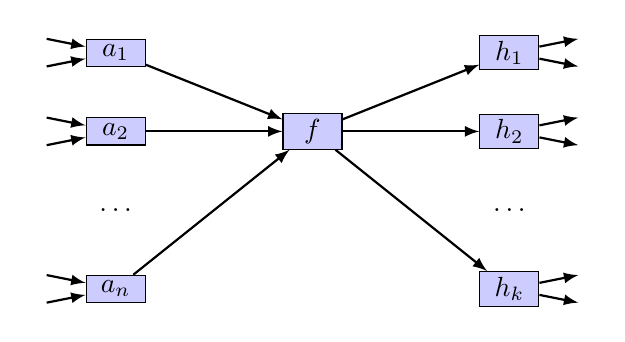
\begin{tikzpicture}
				%\node (a1) [draw, circle, inner sep=0pt, minimum width=0.75cm, fill=green!20] {$a_1$};
				\node (a1) [neuron] {$a_1$};
				\node (a2) [neuron, below of=a1] {$a_2$};
				\node (dots1) [below of=a2] {$\ldots$};
				\node (an) [neuron, below of=dots1] {$a_n$};
				
				\node (f) [neuron, right of=a2, xshift=1.5cm] {$f$};
				
				\node (h2) [neuron, right of=f, xshift=1.5cm] {$h_2$};
				\node (h1) [neuron, above of=h2] {$h_1$};
				\node (dots2) [below of=h2] {$\ldots$};
				\node (hk) [neuron, below of=dots2] {$h_k$};
				
				% inputs
				\node (a1in1) [left of=a1, yshift=0.2cm] {};
				\node (a1in2) [left of=a1, yshift=-0.2cm] {};
				
				\node (a2in1) [left of=a2, yshift=0.2cm] {};
				\node (a2in2) [left of=a2, yshift=-0.2cm] {};
				
				\node (anin1) [left of=an, yshift=0.2cm] {};
				\node (anin2) [left of=an, yshift=-0.2cm] {};
				
				% outputs
				\node (h1o1) [right of=h1, yshift=0.2cm] {};
				\node (h1o2) [right of=h1, yshift=-0.2cm] {};
				
				\node (h2o1) [right of=h2, yshift=0.2cm] {};
				\node (h2o2) [right of=h2, yshift=-0.2cm] {};
				
				\node (hko1) [right of=hk, yshift=0.2cm] {};
				\node (hko2) [right of=hk, yshift=-0.2cm] {};
				
				
				\begin{scope}[thick, black, ->, >=latex]
					\draw (a1) -- (f);
					\draw (a2) -- (f);
					\draw (an) -- (f);
					\draw (f) -- (h1);
					\draw (f) -- (h2);
					\draw (f) -- (hk);
					
					\draw (a1in1) -- (a1);
					\draw (a1in2) -- (a1);
					\draw (a2in1) -- (a2);
					\draw (a2in2) -- (a2);
					\draw (anin1) -- (an);
					\draw (anin2) -- (an);
					
					\draw (h1) -- (h1o1);
					\draw (h1) -- (h1o2);
					\draw (h2) -- (h2o1);
					\draw (h2) -- (h2o2);
					\draw (hk) -- (hko1);
					\draw (hk) -- (hko2);
				\end{scope}	
			\end{tikzpicture}
		}
	\end{figure}
	
	
	Assuming the graph is a function $e = g(\ldots)$, we compute
	$$\pdv{e}{f} = \sum_{i = 1}^{k} \pdv{e}{h_i} \cdot \pdv{h_i}{f}$$
	and
	$$\pdv{f}{a_i} \quad \text{for } a_i, \ldots, a_n$$
	
\end{frame}

\begin{frame}{What each node must implement?}
	
	For example a function $s = f(a, b, c, d)$
	
	\begin{itemize}
		\item How to compute the output value $s$ (given the parameters $a, b, c, d$)
		\item How to compute partial derivatives wrt.\ the parameters, i.e. $\pdv{s}{a}, \pdv{s}{b}, \pdv{s}{c}, \pdv{s}{d}$
	\end{itemize}
	
\end{frame}

\begin{frame}{Backpropagation}
	
	\begin{itemize}
		\item Forward computation: Compute all nodes' output (and cache it)
		\item Backward computation (Backprop): Compute the overall function's partial derivative with respect to each node
	\end{itemize}
	
	\bigskip
	
	Ordering of the computations? Recursively or build a graph's topology upfront and iterate
	
\end{frame}


\begin{frame}{Backpropagation: Recap}
	\begin{itemize}
		\item We can express any arbitrarily complicated function $f: \mathbb{R}^n \to \mathbb{R}$ as a computational graph
		\item For computing the gradient $\nabla f$ at a concrete point $(x_1, x_2, \ldots, x_n)$ we run the forward pass and backprop
		\item When caching each node's intermediate output and partial derivatives, we avoid repeating computations $\to$ efficient algorithm
	\end{itemize}
\end{frame}



\begin{frame}{Take aways}
	
	\begin{itemize}
		
		\item We can quite efficiently find a minimum of any differentiable nested multivariate function
		\begin{itemize}
			\item Iterative gradient descent takes the most promising direction
			\item Backpropagation utilizes computational graphs and caching $\to$ computes gradients efficiently
		\end{itemize}
	\end{itemize}
	
\end{frame}





\section{Text classification}

\begin{frame}{What are we going to achieve}
Example task: Binary sentiment classification into positive and negative

Recall the IMDB dataset

We will learn a simple yet powerful supervised machine learning model

\begin{itemize}
	\item Known as logistic regression, maximum entropy classifier
	\item In fact, it is a single-layer neural network
	\item An essential important building block of deep neural networks
\end{itemize}


\end{frame}



\begin{frame}{High-dimensional linear functions}
Function $f(\bm{x}) : \mathbb{R}^{d_{in}} \to \mathbb{R}^{d_{out}}$
$$f(\bm{x}) \text{ or }
f(\bm{x}; \underbrace{\bm{W}, \bm{b}}_{\mathclap{\text{Explicit parameters}}})
= \bm{x} \bm{W} + \bm{b}$$
where
$\bm{x} \in \mathbb{R}^{d_{in}} \qquad
\bm{W} \in \mathbb{R}^{d_{in} \times d_{out}} \qquad
\bm{b} \in \mathbb{R}^{d_{out}}$

Vector $\bm{x}$ is the \textbf{input}, matrix $\bm{W}$ and vector $\bm{b}$ are the \textbf{parameters} --- typically denoted $\Theta = \bm{W}, \bm{b}$

\begin{block}{Goal of learning}
Find $\bm{W}$ and $\bm{b}$ such that
the function behaves as intended on a collection of input values
$\bm{x}_{1:k} = \bm{x}_1, \ldots, \bm{x}_k$ 
and the corresponding desired outputs
$\bm{y}_{1:k} = \bm{y}_1, \ldots, \bm{y}_k$
\end{block}

\end{frame}




\begin{frame}{Binary classification}

Function $f(\bm{x}) : \mathbb{R}^{d_{in}} \to \mathbb{R}$
$$f(\bm{x}) \text{ or }
f(\bm{x}; \underbrace{\bm{w}, \bm{b}}_{\mathclap{\text{Explicit parameters}}})
= \bm{x} \cdot \bm{w} + b$$

However, for binary text classification
\begin{itemize}
	\item Our input is in the form of a natural language text
	\item Our labels are two categories, e.g., positive and negative
\end{itemize}

\begin{block}{Let's start with the labels}
Very easy: Just arbitrarily map the categories into $0$ and $1$ (e.g., negative = $0$, positive = $1$)
\end{block}

\end{frame}



\section{Numerical representation of natural language text}


\begin{frame}{Goal: Transform text into a fixed-size vector of real numbers}

What's our setup:
$$f(\bm{x}) : \mathbb{R}^{d_{in}} \to \mathbb{R} \qquad
f(\bm{x}) = \bm{x} \cdot \bm{w} + b$$

What we need:
$$\bm{x} \in \mathbb{R}^{d_{in}}$$

What we have:

\emph{One of my favorite movies ever,The Shawshank Redemption is a modern day classic as it tells the story of two inmates who become friends and find solace over the years in which this movie takes place.Based on a Stephen King novel, ...}

\end{frame}


\begin{frame}{What is a ``word''?}

A matter of debate among linguists

Very simplistic definition: words are sequences of letters separated by whitespace

But: \texttt{dog}, \texttt{dog?}, \texttt{dog.}, and \texttt{dog)} would be different words

Better: words separated by whitespace or punctuation

A process called \textbf{tokenization} splits text into tokens based on whitespace and punctuation

\begin{itemize}
	\item English: the job of the tokenizer is quite simple
	\item Hebrew, Arabic: sometimes without whitespace
	\item Chinese: no whitespaces at all
\end{itemize}


\begin{tikzpicture}[overlay, remember picture] 
	\node at (current page.north east)[ref] {\fullcite{Goldberg.2017} \par};
\end{tikzpicture}

\end{frame}

\begin{frame}{Tokens}
	
Symbols \texttt{cat} and \texttt{Cat} have the same meaning, but are they the same word?

Something like \texttt{New York}, is it two words, or one?

\begin{itemize}
	\item We distinguish between words and tokens
	\item We refer to the output of a tokenizer as a token, and to the meaning-bearing units as words
\end{itemize}

\begin{block}{Keep in mind}
We use the term \textbf{word} very loosely, and take it to be interchangeable with \textbf{token}.

In reality, the story is more complex than that.	
\end{block}
	
\end{frame}



\begin{frame}{Vocabulary}

We build a fix-sized static \textbf{vocabulary} (e.g., by tokenizing training data)

\begin{itemize}
	\item Typical sizes: 20,000 -- 100,000 words
\end{itemize}

\bigskip

Each word has a unique fixed index
$$
V = \begin{pmatrix}
\text{a}_1 & \text{abandon}_2 & \ldots & \text{cat}_{852} & \ldots & \text{zone}_{2,999} & \text{zoo}_{3,000}
\end{pmatrix}
$$

\end{frame}

\begin{frame}{(Averaged) Bag-of-words}
$$
\bm{x} = \frac{1}{|D|} \sum_{i =1}^{|D|} \bm{x}^{D_{[i]}}
$$
$D_{[i]}$ -- word in doc $D$ at position $i$, $\bm{x}^{D_{[i]}}$ -- one-hot vector

\begin{block}{Example: a cat sat $\to$ \texttt{a}, \texttt{cat}, \texttt{sat}}
$
V = \begin{pmatrix}
	\text{a}_1 & \text{abandon}_2 & \ldots & \text{cat}_{852} & \ldots & \text{zone}_{2,999} & \text{zoo}_{3,000}
\end{pmatrix}
$
$
\begin{aligned}
\text{a} & = \bm{x}^{D_{[1]}} =
\begin{pmatrix}
1_1 & 0_2 & 0_3 & \ldots & 0_{2,999} & 0_{3,000}
\end{pmatrix} \\
\text{cat} &= \bm{x}^{D_{[2]}} =
\begin{pmatrix}
0_1 & \ldots & 1_{852} & \ldots & 0_{2,999} & 0_{3,000}
\end{pmatrix} \\
\text{sat} &= \bm{x}^{D_{[3]}} =
\begin{pmatrix}
0_1 & \ldots & 1_{2,179} & \ldots & 0_{2,999} & 0_{3,000}
\end{pmatrix}
\end{aligned}
$



	
\end{block}

	
\end{frame}


\begin{frame}{Averaged bag-of-words example: $\bm{x} \in \mathbb{R}^{3,000}$}

\begin{block}{Example: a cat sat $\to$ \texttt{a}, \texttt{cat}, \texttt{sat}}

$
\begin{aligned}
	\text{a} & = \bm{x}^{D_{[1]}} =
	\begin{pmatrix}
		1_1 & 0_2 & 0_3 & \ldots & 0_{2,999} & 0_{3,000}
	\end{pmatrix} \\
	\text{cat} &= \bm{x}^{D_{[2]}} =
	\begin{pmatrix}
		0_1 & \ldots & 1_{852} & \ldots & 0_{2,999} & 0_{3,000}
	\end{pmatrix} \\
	\text{sat} &= \bm{x}^{D_{[3]}} =
	\begin{pmatrix}
		0_1 & \ldots & 1_{2,179} & \ldots & 0_{2,999} & 0_{3,000}
	\end{pmatrix}
\end{aligned}
$
	
\end{block}
$$
\begin{aligned}
\bm{x} &= \frac{1}{|D|} \sum_{i =1}^{|D|} \bm{x}^{D_{[i]}} \\
&= \begin{pmatrix}
	0.33_1 & 0_2 & \ldots & 0_{851} & 0.33_{852} & 0_{853} & \ldots & 0.33_{2,179} & \ldots & 0_{3,000}
\end{pmatrix}	
\end{aligned}
$$
	

		
\end{frame}


\begin{frame}{Out-of-vocabulary (\texttt{UNK}) tokens}
	
Words in a language are very unevenly distributed

\begin{itemize}
	\item There is always a large `tail' of rare words
\end{itemize}

When building the vocabulary, use the most frequent words, all others represented by an unknown token (\texttt{UNK} or \texttt{OOV})


\begin{block}{Example vocabulary, most common 3,000 words and \texttt{UNK}}
$
V = \begin{pmatrix}
	\text{a}_1 & \text{abandon}_2 & \ldots & \text{zone}_{2,999} & \text{zoo}_{3,000} & \text{UNK}_{3,001}
\end{pmatrix}
$
\end{block}

\begin{itemize}
	\item In machine translation, how to translate the \texttt{UNK} word?
\end{itemize}

\begin{tikzpicture}[overlay, remember picture] 
	\node at (current page.north east)[ref] {\fullcite{Koehn.2020} \par};
\end{tikzpicture}

\end{frame}


\begin{frame}{Subword units: Byte-pair encoding}

\begin{enumerate}
	\item The words in the corpus are split into characters (marking original spaces with a special space character) --- this is the initial vocabulary $V$
	\item The most frequent pair of characters is merged and added to $V$
	\item Repeat 2 for a fixed given number of times
	\item Each of these steps increases $V$ by one, beyond the original inventory of single characters
\end{enumerate}

When done over large corpora with multiple languages and writing systems, BPE prevents OOV!

\end{frame}


\begin{frame}{Byte-pair encoding example on a toy corpus (part 1)}

\small{
\texttt{t h i s \_ f a t \_ c a t \_ w i t h \_ t h e \_ h a t \_ i s \_ i n \_ t h e \_ c a v e  \_ o f \_ t h e \_ t h i n \_ b a t}
}

Most frequent: \texttt{t h} (6 times), merge into a single token

\small{
\texttt{th i s \_ f a t \_ c a t \_ w i th \_ th e \_ h a t \_ i s \_ i n \_ th e \_ c a v e  \_ o f \_ th e \_ th i n \_ b a t}
}

Most frequent: \texttt{a t} (4 times), merge into a single token

\small{
\texttt{th i s \_ f at \_ c at \_ w i th \_ th e \_ h at \_ i s \_ i n \_ th e \_ c a v e  \_ o f \_ th e \_ th i n \_ b at}
}


\end{frame}

\begin{frame}{Byte-pair encoding example on a toy corpus (part 2)}

\small{	
\texttt{th i s \_ f at \_ c at \_ w i th \_ th e \_ h at \_ i s \_ i n \_ th e \_ c a v e  \_ o f \_ th e \_ th i n \_ b at}
}

Most frequent: \texttt{th e} (3 times), merge into a single token

\small{
\texttt{th i s \_ f at \_ c at \_ w i th \_ the \_ h at \_ i s \_ i n \_ the \_ c a v e  \_ o f \_ the \_ th i n \_ b at}
}

\small{
$V = \{
\text{\texttt{t, h, i, s, \_, f, a, c, w, e, n, v, o, f, b, th, at, the}}
\}$
}


\begin{tikzpicture}[overlay, remember picture] 
	\node at (current page.north east)[anchor = north east, text width=4cm, yshift=-1.3cm] {\scriptsize At the end of this process, the most frequent words will emerge as single tokens, while rare words consist of still unmerged subwords \par};
\end{tikzpicture}	

\end{frame}

\begin{frame}{SentencePiece: A variant of byte pair encoding}

\begin{block}{Byte-pair example. Word splits indicated with \texttt{@@}.}
\texttt{[the] [relationship] [between] [Obama] [and] [Net@@] [any@@] [ahu] [is] [not] [exactly] [friendly] [.]}
\end{block}

SentencePiece escapes the whitespace with \texttt{\_} and tokenizes the input into an arbitrary subword sequence

\begin{block}{SentencePiece example of "Hello world."}
\texttt{[Hello] [\_wor] [ld] [.]}
\end{block}

Lossless tokenization --- all the information to reproduce the normalized
text is preserved

\begin{tikzpicture}[overlay, remember picture] 
	\node at (current page.north east)[ref] {\fullcite{Kudo.Richardson.2018.EMNLP} \par};
\end{tikzpicture}

\end{frame}

\begin{frame}{Recap: Transform text into a fixed-size vector of real numbers}
	
What's our setup:
$$f(\bm{x}) : \mathbb{R}^{d_{in}} \to \mathbb{R} \qquad
f(\bm{x}) = \bm{x} \cdot \bm{w} + b$$

What we need:
$$\bm{x} \in \mathbb{R}^{d_{in}}$$
	
What we have:
	
\emph{One of my favorite movies ever,The Shawshank Redemption is a modern day classic  ...}

Simple solution:

\begin{itemize}
	\item Bag-of-words (tokenized), $d_{in} = |V|$
\end{itemize}
	
\end{frame}




\section{Binary text classification}


\subsection{Binary classification as a function}

\begin{frame}{Linear function and its derivatives}
	
We have this linear function
$$f(\bm{x}) : \mathbb{R}^{d_{in}} \to \mathbb{R} \qquad
f(\bm{x}) = \bm{x} \cdot \bm{w} + b = \bm{x}_{[1]} \bm{w}_{[1]} + \ldots + \bm{x}_{[d_{in}]} \bm{w}_{[d_{in}]} + b $$

\begin{block}{Derivatives wrt.\ parameters $\bm{w}$ and $b$}
$$
\dv{f}{\bm{w}_{[i]}} = \bm{x}_{[i]} \qquad \dv{f}{b} = 1
$$
\end{block}


\end{frame}


\begin{frame}{Non-linear mapping to $[0, 1]$}

We have this linear function
$$f(\bm{x}) : \mathbb{R}^{d_{in}} \to \mathbb{R} \qquad
f(\bm{x}) = \bm{x} \cdot \bm{w} + b$$
which has an unbounded range $(-\infty, +\infty)$

\bigskip

However, each example's label is $y \in \{0, 1\}$

\end{frame}


\begin{frame}{Sigmoid (logistic) function}

\begin{block}{Sigmoid function $\sigma(t) : \mathbb{R} \to \mathbb{R}$}
	$$
	\sigma(t) = \frac{\exp(t)}{\exp(t) + 1} = \frac{1}{1 + \exp(-t)}
	$$
\end{block}


\begin{figure}
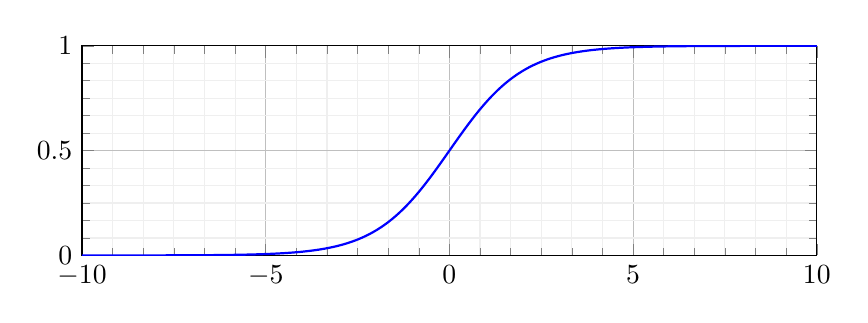
\begin{tikzpicture}

\begin{axis}[
	xmin = -10, xmax = 10,
	ymin = 0, ymax = 1,
	xtick distance = 5,
	ytick distance = 0.5,
	grid = both,
	minor tick num = 5,
	major grid style = {lightgray},
	minor grid style = {lightgray!25},
	width = 0.9\textwidth,
	height = 0.35\textwidth,
	legend pos = north west
	]
	
	\addplot[
	domain = -10:10,
	samples = 200,
	smooth,
	thick,
	blue,
	] {1/(1 + exp(-1 * x))};
	
\end{axis}
\end{tikzpicture}
\end{figure}

Symmetric function, range of $\sigma(t) \in [0, 1]$, 

	
\end{frame}

\begin{frame}{Sigmoid $\sigma(t) = \frac{1}{1 + \exp(-t)}$}

\begin{block}{Derivative of sigmoid wrt.\ its input}
$$
\begin{aligned}
\dv{\sigma}{t}
&=\frac {\exp(t) \cdot (1+\exp(t)) - \exp(t) \cdot \exp(t)}{(1+\exp(t))^{2}} \\
&= \ldots \\
&= \sigma(t) \cdot \left( 1- \sigma(t) \right)
\end{aligned}
$$	
\end{block}



\end{frame}

\begin{frame}{Our binary text classification function}

Linear function through sigmoid --- log-linear model
$$
\hat{y} = \sigma(f(\bm{x})) = \frac{1}{1 + \exp(- (\bm{x} \cdot \bm{w} + b))}
$$	

\begin{figure}
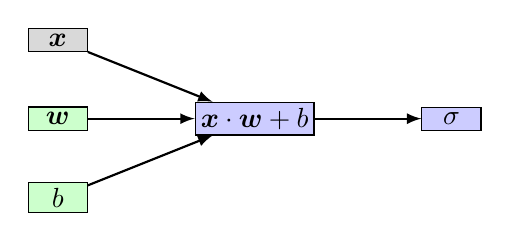
\begin{tikzpicture}	
	%\node (a1) [draw, circle, inner sep=0pt, minimum width=0.75cm, fill=green!20] {$a_1$};
	\node (x) [constant] {$\bm{x}$};
	\node (w) [param, below of=x] {$\bm{w}$};
	\node (b) [param, below of=w] {$b$};
	
	\node (f) [neuron, right of=w, xshift=1.5cm] {$\bm{x} \cdot \bm{w} + b$};
	\node (s) [neuron, right of=f, xshift=1.5cm] {$\sigma$};
	
	\begin{scope}[thick, black, ->, >=latex]
		\draw (x) -- (f);
		\draw (w) -- (f);
		\draw (b) -- (f);
		\draw (f) -- (s);
	\end{scope}	
\end{tikzpicture}
\caption{Computational graph; green nodes are trainable parameters, gray are inputs}
\end{figure}
	
\end{frame}

\begin{frame}{Decision rule of log-linear model}
	
Log-linear model
$
\hat{y} = \sigma(f(\bm{x})) = \frac{1}{1 + \exp(- (\bm{x} \cdot \bm{w} + b))}
$	

\begin{itemize}
	\item Prediction = 1 if $\hat{y} > 0.5$	
	\item Prediction = 0 if $\hat{y} < 0.5$
\end{itemize}

\bigskip

Natural interpretation: Conditional probability of prediction = 1 given the input $\bm{x}$
$$
\begin{aligned}
\sigma(f(\bm{x})) &= \Pr(\text{prediction} = 1 | \bm{x}) \\
1 - \sigma(f(\bm{x})) &= \Pr(\text{prediction} = 0 | \bm{x})
\end{aligned}
$$

\end{frame}

\subsection{Finding the best model's parameters}



\begin{frame}{Binary cross-entropy loss (logistic loss)}
$$
L_{\text{logistic}} = - y \log \hat{y} - (1 - y) \log (1 - \hat{y})
$$

\begin{block}{Partial derivative wrt.\ input $\hat{y}$}
$$
\dv{L_{\text{Logistic}}}{\hat{y}} =
- \left(
\frac{y}{\hat{y}} - \frac{1 - y}{1 - \hat{y}}
\right)
=
- \frac{y - \hat{y}}{ \hat{y} (1 - \hat{y})}
$$
\end{block}

\end{frame}

\begin{frame}{Full computational graph}
\begin{figure}
	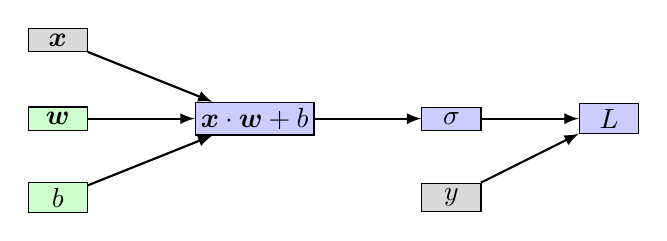
\begin{tikzpicture}	
		%\node (a1) [draw, circle, inner sep=0pt, minimum width=0.75cm, fill=green!20] {$a_1$};
		\node (x) [constant] {$\bm{x}$};
		\node (w) [param, below of=x] {$\bm{w}$};
		\node (b) [param, below of=w] {$b$};
		
		\node (f) [neuron, right of=w, xshift=1.5cm] {$\bm{x} \cdot \bm{w} + b$};
		\node (s) [neuron, right of=f, xshift=1.5cm] {$\sigma$};
		
		\node (l) [neuron, right of=s, xshift=1cm] {$L$};
		\node (y) [constant, below of=s] {$y$};
		
		\begin{scope}[thick, black, ->, >=latex]
			\draw (x) -- (f);
			\draw (w) -- (f);
			\draw (b) -- (f);
			\draw (f) -- (s);
			\draw (s) -- (l);
			\draw (y) -- (l);
		\end{scope}	
	\end{tikzpicture}
	\caption{Computational graph; green nodes are trainable parameters, gray are constant inputs}
\end{figure}

How can we minimize this function?

\begin{itemize}
	\item Recall: (a) Gradient descent and (b) backpropagation
\end{itemize}

\end{frame}

\begin{frame}{(Online) Stochastic Gradient Descent}

\begin{algorithmic}[1]
	\Function{SGD}{$f(\bm{x}; \Theta)$, $(\bm{x}_1, \ldots, \bm{x}_n)$, $(\bm{y}_1, \ldots, \bm{y}_n)$, $L$}
	\While{stopping criteria not met}
		\State Sample a training example $\bm{x}_i, \bm{y}_i$
		\State Compute the loss $L(f(\bm{x}_i; \Theta), \bm{y}_i)$
		\State $\hat{\bm{g}} \gets$ gradient of $L(f(\bm{x}_i; \Theta), \bm{y}_i)$ wrt.\ $\Theta$
		\State $\Theta \gets \Theta - \eta_t \hat{\bm{g}}$
	\EndWhile
	\State \Return $\Theta$
	\EndFunction
\end{algorithmic}

Loss in line 4 is based on a \textbf{single training example} $\to$ a rough estimate of the corpus loss $\mathcal{L}$ we aim to minimize

The noise in the loss computation may result in inaccurate gradients

\end{frame}



\begin{frame}{Minibatch Stochastic Gradient Descent}
	
	\begin{algorithmic}[1]
		\Function{mbSGD}{$f(\bm{x}; \Theta)$, $(\bm{x}_1, \ldots, \bm{x}_n)$, $(\bm{y}_1, \ldots, \bm{y}_n)$, $L$}
		\While{stopping criteria not met}
		\State Sample $m$ examples $\{ (\bm{x}_1, \bm{y}_1), \ldots (\bm{x}_m, \bm{y}_m) \}$
		\State $\hat{\bm{g}} \gets 0$
		\For{$i = 1$ to $m$}
			\State Compute the loss $L(f(\bm{x}_i; \Theta), \bm{y}_i)$
			\State $\hat{\bm{g}} \gets \hat{\bm{g}}\ + $ gradient of $\frac{1}{m} L(f(\bm{x}_i; \Theta), \bm{y}_i)$ wrt.\ $\Theta$
		\EndFor
		\State $\Theta \gets \Theta - \eta_t \hat{\bm{g}}$
		\EndWhile
		\State \Return $\Theta$
		\EndFunction
	\end{algorithmic}
	

\end{frame}

\begin{frame}{Properties of Minibatch Stochastic Gradient Descent}

The minibatch size can vary in size from $m = 1$ to $m = n$

Higher values provide better estimates of the corpus-wide gradients, while smaller values allow more updates and in turn faster convergence

Lines 6+7: May be easily parallelized

\end{frame}



\section*{Recap}

\begin{frame}{Take aways}
	
\begin{itemize}
	\item Tokenization is tricky	
	\item Simplest representation of text as bag-of-word features
	\item Binary classification as a linear function of words and a sigmoid
	\item Binary cross-entropy (logistic) loss
	\item Training as minimizing the loss using minibatch SGD and backpropagation
\end{itemize}
	
\end{frame}









\begin{frame}{License and credits}
	
	\begin{columns}
		\begin{column}{0.7\textwidth}
			Licensed under Creative Commons Attribution-ShareAlike 4.0 International (CC BY-SA 4.0)
		\end{column}
		\begin{column}{0.2\textwidth}
			\includegraphics[width=0.9\linewidth]{img/cc-by-sa-icon.pdf}
		\end{column}
	\end{columns}
	
	\bigskip
	
	Credits
	
	\begin{scriptsize}
		
		Ivan Habernal
		
		Content from ACL Anthology papers licensed under CC-BY \url{https://www.aclweb.org/anthology}
		
	\end{scriptsize}
	
\end{frame}


\appendix

\section*{Appendix}


\begin{frame}{Mathematical notation}

\begin{block}{Scalars, vectors, matrices}

Lowercase letters represent scalars: $x, y, b$
	
Bold lowercase letters represent vectors: $\bm{w}, \bm{x}, \bm{b}$

Bold uppercase letters represent matrices: $\bm{W}, \bm{X}$

\end{block}

\begin{block}{Indexing}
	
$[ . ]$ as the index operator of vectors and matrice

$\bm{b}_{[i]}$ is the $i$-th element of vector $\bm{b}$

$\bm{W}_{[i,j]}$ is the $i$-th row, $j$-th column of matrix $\bm{W}$
\end{block}

\end{frame}


\begin{frame}{Notation}
	
\begin{block}{Sequences}

$\bm{x}_{1:n}$ is a sequence of vectors $\bm{x}_1, \ldots, \bm{x}_n$

$[\bm{v}_1 ; \bm{v}_2]$ is vector concatenation
	
\end{block}
	
\begin{block}{Note! We use vectors as \emph{row} vectors}
%Unless otherwise stated, vectors are (somewhat unorthodox) \textbf{row} vectors
$$
\bm{x} \in \mathbb{R}^{d}
$$
\end{block}

Example $d = 5$:
$$
\bm{x} = \begin{pmatrix}
1 & 2 & 3 & 4 & 5
\end{pmatrix}
$$
which is simply a list (1-d array) of numbers $(1, 2, 3, 4, 5)$

\end{frame}

\begin{frame}{Multiplication example}
	
$$
\bm{x} \in \mathbb{R}^{d_{in}} \qquad
\bm{W} \in \mathbb{R}^{d_{in} \times d_{out}} \qquad
\bm{b} \in \mathbb{R}^{d_{out}}
$$


\begin{block}{Example: $\bm{y} = \bm{x} \bm{W} + \bm{b}$, $d_{in} = 3$, $d_{out} = 2$}
	$$
	\begin{pmatrix}
		\bm{x}_{[1]} & \bm{x}_{[2]} & \bm{x}_{[3]}
	\end{pmatrix}
	\begin{pmatrix}
		\bm{W}_{[1,1]} & \bm{W}_{[1,2]} \\
		\bm{W}_{[2,1]} & \bm{W}_{[2,2]} \\
		\bm{W}_{[3,1]} & \bm{W}_{[3,2]} \\
	\end{pmatrix}
	+
	\begin{pmatrix}
		\bm{b}_{[1]} & \bm{b}_{[2]}
	\end{pmatrix}
	=
	\begin{pmatrix}
		\bm{y}_{[1]} & \bm{y}_{[2]}
	\end{pmatrix}
	$$
\end{block}
	
\end{frame}



\begin{frame}{Mult.\ simplified with dot product $\bm{u} \cdot \bm{v} = \sum_i \bm{u}_{[i]} \bm{v}_{[i]}$}
	
\begin{block}{Example: $\bm{y} = \bm{x} \bm{W} + \bm{b}$, $d_{in} = 3$, $d_{out} = 1$}
$\bm{x} \in \mathbb{R}^{d_{in}} \qquad
\bm{W} \in \mathbb{R}^{d_{in} \times d_{out}} \qquad
\bm{b} \in \mathbb{R}^{d_{out}}$
	$$
	\begin{pmatrix}
		\bm{x}_{[1]} & \bm{x}_{[2]} & \bm{x}_{[3]}
	\end{pmatrix}
	\begin{pmatrix}
		\bm{W}_{[1,1]}  \\
		\bm{W}_{[2,1]}  \\
		\bm{W}_{[3,1]}  \\
	\end{pmatrix}
	+ b
	= y
	$$
\end{block}


\begin{block}{Equivalent dot product: $y = \bm{x} \cdot \bm{w} + b$, $d_{in} = 3$, $d_{out} = 1$}
$\bm{x} \in \mathbb{R}^{d_{in}} \qquad
\bm{w} \in \mathbb{R}^{d_{out}} \qquad
b \in \mathbb{R}$
	$$
	\begin{pmatrix}
		\bm{x}_{[1]} & \bm{x}_{[2]} & \bm{x}_{[3]}
	\end{pmatrix}
	\cdot
	\begin{pmatrix}
		\bm{w}_{[1]} & \bm{w}_{[2]} & \bm{w}_{[3]}
	\end{pmatrix}
	+ b
	= y
	$$
\end{block}

\end{frame}




\end{document}

